
%%%%%%%%%%%%%  Start of GENERATED TEXT  %%%%%%%%%%%%\n

\newpage
\setcounter{page}{1}
\setcounter{section}{0}
\setcounter{equation}{0}
\setcounter{figure}{0}
\setcounter{table}{0}
\setcounter{footnote}{0}
\renewcommand{\ehkol}{Kolomiiets B. Yu., Karplyuk Ye. S.}
\renewcommand{\ohkol}{Improving sEMG Gesture Classification with Transfer Learning: Accuracy, Stability, and Low-Data Adaptation}
\Vykh{radap20NN:FirstPage}{radap20NN:LastPage}
\begin{multicols}{2}
[
\UDC{}
\renewcommand{\ehkol}{Kolomiiets B. Yu., Karplyuk Ye. S.}
\renewcommand{\ohkol}{Improving sEMG Gesture Classification with Transfer Learning: Accuracy, Stability, and Low-Data Adaptation}
\Title{Improving sEMG Gesture Classification with Transfer Learning: Accuracy, Stability, and Low-Data Adaptation}\label{radap20NN:FirstPage}
\Authors{Kolomiiets B. Yu., Karplyuk Ye. S.}
\aff{National Technical University of Ukraine "Igor Sikorsky Kyiv Polytechnic Institute", Kyiv, Ukraine}
\Address{}{kolomiiets.bohdan.yuriyovych@gmail.com}
\AbsKeywords{
Surface electromyography (sEMG) enables intuitive and non-invasive human–machine interfacing, yet its practical deployment remains limited by inter-subject variability and the substantial effort required for subject-specific model calibration. In this work, we evaluate the effectiveness of transfer learning to address these challenges in the context of deep learning-based gesture classification, using a dataset that includes eleven gestures repeated eight times by 22 subjects. We systematically compare three training paradigms: (i) intra-subject training, (ii) inter-subject generalization, and (iii) transfer learning with and without resetting the classifier’s fully connected (FC) output layer. A rigorous leave-one-out cross-validation scheme was applied across all subjects and repetitions to ensure robust evaluation.
Our results show that both transfer learning strategies outperform baseline models in terms of classification accuracy, with the best performance achieved when fine-tuning with a reset FC layer (F1-score = 0.907, $\sigma = 0.074$). Statistical analysis using Wilcoxon signed-rank tests confirms that these improvements are significant, even when only a limited number of subject-specific repetitions are used for fine-tuning. Notably, the transfer learning approach being trained on four repetitions maintains almost the same performance compared to training from scratch on eight repetitions, halving training repetitions while preserving accuracy. This represents a substantial reduction in calibration effort without sacrificing performance.
These findings support the use of pre-trained models for rapid subject adaptation in sEMG-controlled systems and validate fine-tuning with FC reset as an effective strategy for improving both performance and model stability. The methodology and results presented in this work contribute to the development of practical, adaptive, and low-effort EMG-based interfaces for assistive and rehabilitative applications.
}
{Keywords}{
surface electromyography (sEMG), gesture recognition, transfer learning, deep learning, convolutional neural networks (CNN), inter-subject variability, model generalization, fine-tuning strategies, subject adaptation, myoelectric control, EMG-based interface, cross-validation, biomedical signal processing, rehabilitation technologies, low-effort calibration
 }
{\href{http://radap.kpi.ua/radiotechnique/article/view/20NN}{10.20535/RADAP.2025.\#\#.\pageref{radap20NN:FirstPage}-\pageref{radap20NN:LastPage}}}
]

%
%

\pdfbookmark[1]{Introduction}{intro}
\section*{Introduction}

Surface electromyography (sEMG) is a non-invasive technique for monitoring the electrical activity generated by muscle contractions, with significant applications in rehabilitation, prosthetics, assistive robotics, and human–computer interaction~\cite{Zhou2023}. sEMG signals are widely used to facilitate gesture recognition, control of prosthetic limbs, and functional recovery assessment in neuromuscular disorders~\cite{Xie2024}.

However, the utility of sEMG is constrained by several physiological and technical factors. One of the most critical is electrode placement. Minor changes in electrode positioning can result in substantial variations in signal amplitude and frequency content due to anatomical and physiological variability~\cite{Merletti2020}. In addition, factors like skin impedance, muscle fatigue, and motion artifacts further degrade signal quality~\cite{Plux2022}.

Classical signal processing techniques—such as time-domain and frequency-domain analysis, wavelet transforms, and handcrafted feature extraction—have long been employed for EMG interpretation~\cite{Chowdhury2013}. While these methods offer computational efficiency and domain-specific interpretability, they often fall short in capturing the complex spatiotemporal patterns associated with dynamic or multichannel sEMG data. Their generalization performance is also limited, especially across subjects or sessions~\cite{Phinyomark2019}.

The introduction of deep learning, particularly convolutional neural networks (CNNs), has significantly enhanced the capacity to extract meaningful representations from raw EMG data. CNNs enable automatic hierarchical feature learning, yielding improved classification performance compared to traditional machine learning models such as SVMs or decision trees~\cite{Faust2018}. However, CNNs typically require large, well-labeled datasets to generalize effectively—a constraint that remains a significant bottleneck in biomedical applications, where data acquisition is often expensive and time-consuming~\cite{Wu2022}.

To mitigate this, transfer learning has become a popular strategy. It enables the reuse of models pre-trained on larger datasets to improve performance on smaller, task-specific datasets. Several techniques exist, including fine-tuning the entire model, freezing early layers while adapting the classifier head, or applying domain adaptation methods. These strategies have shown varying degrees of success in sEMG classification, depending on the architecture and dataset used~\cite{Cote2019, Ameri2020}.

Furthermore, recent progress in wearable electronics—such as flexible sensors, edge computing modules, and energy-efficient microcontrollers—has made it feasible to deploy deep learning models for real-time sEMG classification. This technological convergence supports the development of intelligent, embedded systems capable of continuous physical activity monitoring and adaptive neurorehabilitation ~\cite{Shen2020}.

Thus, the current research focuses on optimizing the use of transfer learning in CNN-based sEMG gesture classification, particularly evaluating strategies that can enhance performance with limited subject-specific data.

\section{Statement of the Problem}

Although convolutional neural networks (CNNs) have demonstrated considerable success in electromyographic (EMG) gesture recognition, their performance often degrades when applied across different subjects without subject-specific training. This limitation hinders the development of generalizable EMG-based human–machine interfaces that can be deployed without extensive per-user calibration~\cite{Cote2019, Geng2016}.

Transfer learning offers a promising approach to improve generalization by leveraging knowledge learned from one group of subjects and adapting it to another. However, the practical effectiveness of different transfer learning strategies—such as fine-tuning the full model versus using a fixed feature extractor—remains insufficiently explored in the context of sEMG-based gesture recognition~\cite{Lehmler2021}.

Moreover, existing literature rarely compares these strategies systematically on standardized datasets using rigorous evaluation protocols. This lack of comparative insight creates uncertainty around which approach yields better classification performance and model stability, especially when the amount of available target subject data is limited.

This study addresses these gaps by experimentally evaluating and comparing two transfer learning strategies in a real-world sEMG classification scenario: (1) fine-tuning with the reset of the fully connected (FC) output layer and (2) fine-tuning without resetting the FC layer. We assess each method's effect on classification accuracy and result variance using the 3DC dataset~\cite{Cote2019_3DC}. Additionally, we test whether these strategies reduce the quantity of subject-specific training data required while maintaining or improving model performance.

\section{Dataset}

The \textit{3DC Dataset} dataset comprises surface electromyography (sEMG) recordings collected from 22 able-bodied participants performing eleven distinct hand and wrist gestures. Each subject completed eight repetitions of a predefined gesture sequence, resulting in a substantial volume of labeled gesture data.

The 3DC Dataset was introduced in the work by Côté-Allard et al.~\cite{Cote2019_3DC}, where the authors designed a low-cost, 3D-printed, wireless myoelectric armband known as the 3DC Armband. This device features 10 dry sEMG electrodes and a 9-axis inertial measurement unit (IMU), with a sampling rate of 1000 Hz. The data acquisition protocol involved placing the 3DC Armband on the dominant forearm of each participant, alternating the armband's position relative to the elbow between participants to simulate real-world variability in wearability.

Subjects were instructed to perform eleven gestures—such as wrist flexion, extension, and different hand shapes—each held for 5 seconds per repetition. These recordings were organized into eight continuous cycles of data acquisition, separated by a 5-minute rest period between the fourth and fifth cycles.

Due to the diverse electrode placement protocols used in the original study to simulate real-world variability, substantial intra- and inter-subject signal differences are present. One the one hand, it challenges the generalization capability of learned models, and on the other hand - it makes this dataset a good benchmark for evaluating inter-subject generalization and transfer learning strategies in sEMG-based gesture classification.

\section{Methods}

The research was conducted using the \texttt{LibEMG} Python library~\cite{LibEMG2023}, which provides a unified framework for data loading, preprocessing, training, and evaluation of machine learning models in electromyographic control systems.

As recent deep learning studies suggest, the raw sEMG signal can be ingested directly for gesture classification~\cite{Oskoei2007,Rehman2018,Cote2019}.

Adhering to the already existing best-practices~\cite{Smith2011} and works that use chosen dataset~\cite{Cote2019_3DC,LibEMG2023}, in this study, raw EMG signals are split into 200-sample overlapping windows (with a step size of 100) forming matrixes of size $10 \times 200$ that serves as the input to our CNN. 

\subsection*{CNN Architecture}
The CNN architecture used in this study is based on implementations from works~\cite{Cote2019_3DC,LibEMG2023}. 
The final architecture used in this study consists of three sequential 1D convolutional layers followed by a fully connected (FC) output layer. The network was designed to process raw surface EMG input of shape $10 \times 200$ (channels × samples), where each input segment corresponds to a 200-sample window of 10-channel EMG data.
Each convolutional block includes a \texttt{Conv1d} layer with kernel size 5, followed by batch normalization and a ReLU activation function. The number of filters in successive convolutional layers tapers from 64 to 32 and then 16, forming a pyramid structure that progressively condenses features. The output of the final convolutional layer is flattened and passed to a fully connected layer of size 3008 $\rightarrow$ 11, where 11 corresponds to the number of gesture classes.
Weights for all layers were initialized using Glorot (Xavier) uniform initialization, and biases were set to zero. The network was optimized using the Adam optimizer (initial learning rate of $10^{-3}$) with a cosine annealing learning rate schedule and trained using cross-entropy loss. Early stopping was applied with a patience of four epochs and tolerance threshold of 0.03. A maximum of 50 epochs was allowed during training, although convergence typically occurred within 15 epochs. To ensure reproducibility, all random seeds were explicitly set for PyTorch, NumPy, and Python’s built-in generators.
The exact implementation of the CNN used in this study is available in the publicly accessible repository~\cite{Kolomiiets2025}.

\subsection*{Evaluated training approaches}

Three training approaches were evaluated:

\begin{itemize}
    \item \textbf{Intra-subject (single-subject) training}: The model was trained and tested on different gesture repetitions from the same participant. We applied leave-one-out cross-validation strategy for repetitions, choosing one repetition as test set, one repetition as validation set during training, and six for training itself within each subject. Such cross-validation yields 65 folds per subject.
    \item \textbf{Inter-subject (cross-subject) generalization}: The model was trained on 21 subjects and tested on the one excluded subject. The same leave-one-out cross-validation strategy for repetitions was applied per each excluded subject.
    \item \textbf{Transfer learning}: The best pre-trained cross-subject models were fine-tuned on subject-specific data using two strategies: (1) resetting the final FC layer before fine-tuning and (2) preserving the final FC layer weights. All convolutional layers remained trainable during fine-tuning.
\end{itemize}

Additionally, to evaluate whether the transfer learning approach with FC layer reset still outperforms training from scratch—especially when less subject-specific data is available—we repeated the Intra-subject'' and Transfer learning’’ experiments using fewer training repetitions. While the original experiments used 6 out of 8 available repetitions for training, the new experiments were conducted using only 4, 2, and 1 repetitions to simulate more limited data scenarios.

To compare the effectiveness of transfer learning approaches, Wilcoxon signed-rank tests were performed for all experiments.

\section{Results and Discussion}

To evaluate the performance of different training approaches, F1-score was selected as the primary accuracy metric.

Figure~\ref{fig:boxplot-approaches} presents box-and-whisker plots summarizing the F1-score distributions for inter-subject generalization, intra-subject training, and two transfer learning strategies: fine-tuning with and without resetting the fully connected (FC) layer. All eight available repetitions were used for training in those experiments. Consequently, distributions are based on $1232 (8*7*22)$ cross-validation folds per training approach across all 22 subjects.

The inter-subject approach yielded a mean F1-score of 0.382 ($\sigma = 0.149$), confirming that generalization across subjects is significantly limited due to variability in electrode placement and anatomical differences. In contrast, intra-subject training—where the model is trained and tested on data from the same participant—achieved a dramatically higher mean F1-score of 0.869 ($\sigma = 0.089$).

Fine-tuning pre-trained models using the ``without FC reset'' transfer learning strategy further improved performance to 0.896 ($\sigma = 0.071$). However, the best result was obtained using the ``with FC reset'' transfer learning strategy, achieving a mean of 0.907 ($\sigma = 0.074$), suggesting that resetting the CNN's head enables better adaptation to new subjects. Both transfer learning strategies outperformed intra-subject training approach, affirming the benefit of using pre-trained models.

To assess whether transfer learning allowes to reduce the amount of subject-specific data, we additionally performed experiments with decreased numbers of training repetitions (6, 4, 3). As shown in Figure~\ref{fig:boxplot-reps}, the transfer learning approach with FC layer reset consistently achieves higher F1-scores across all scenarios. While reducing the number of training repetitions to three results in a noticeable decline in accuracy, using four repetitions yields only a modest decrease. This effectively halves the required subject effort compared to using all eight repetitions, without substantially compromising classification accuracy.

\end{multicols}

\begin{center}
\centering%{l}{\linewidth}
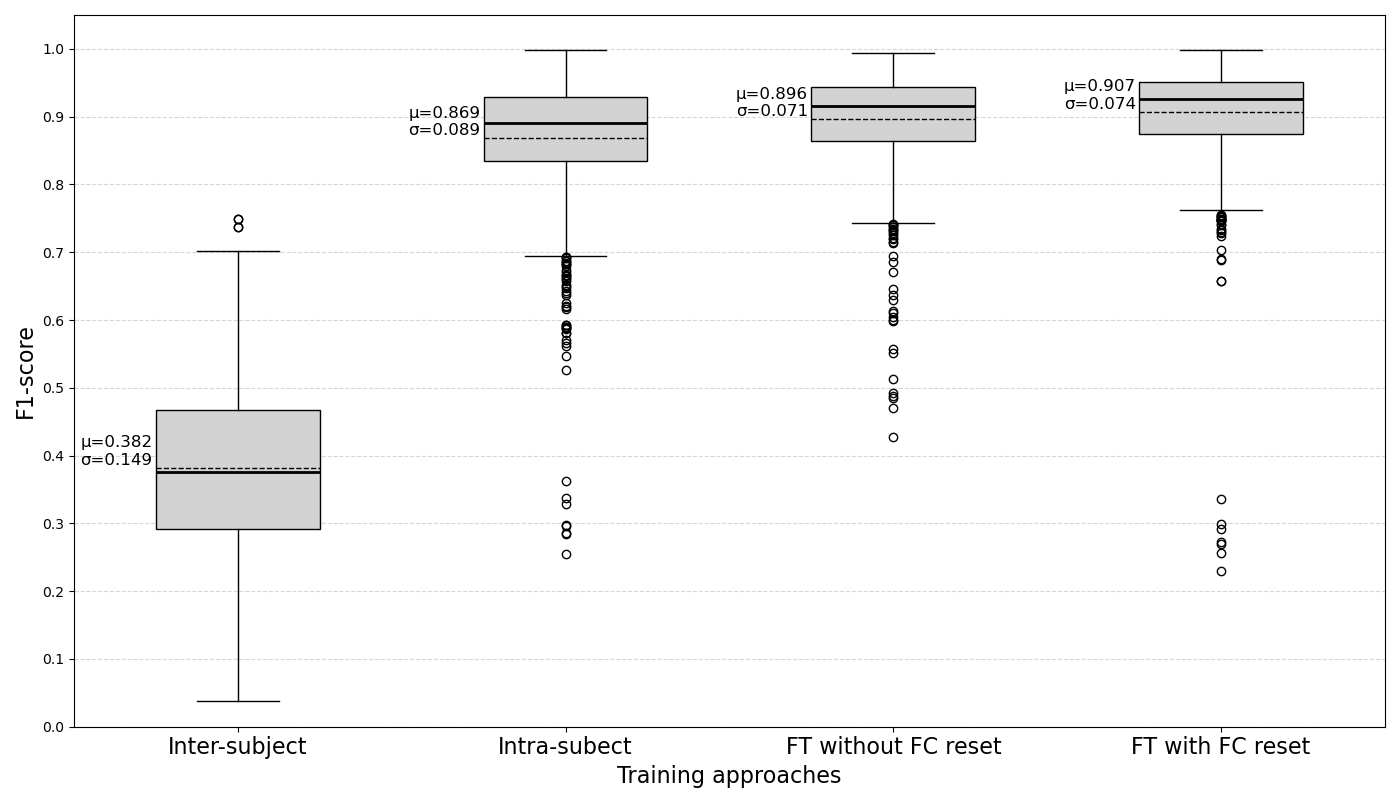
\includegraphics[width=\linewidth]{accuracy_by_approach_8_reps}
\captionof{figure}{Box-and-whisker plots of F1-score distributions across training approaches: inter-subject generalization, intra-subject training, and two variants of transfer learning (with and without fully connected (FC) layer reset). Boxes represent interquartile range (IQR), lines show medians, and dashed lines indicate means. Outliers are shown as individual points.}
\label{fig:boxplot-approaches}
\end{center}

\begin{center}
\centering%{l}{\linewidth}
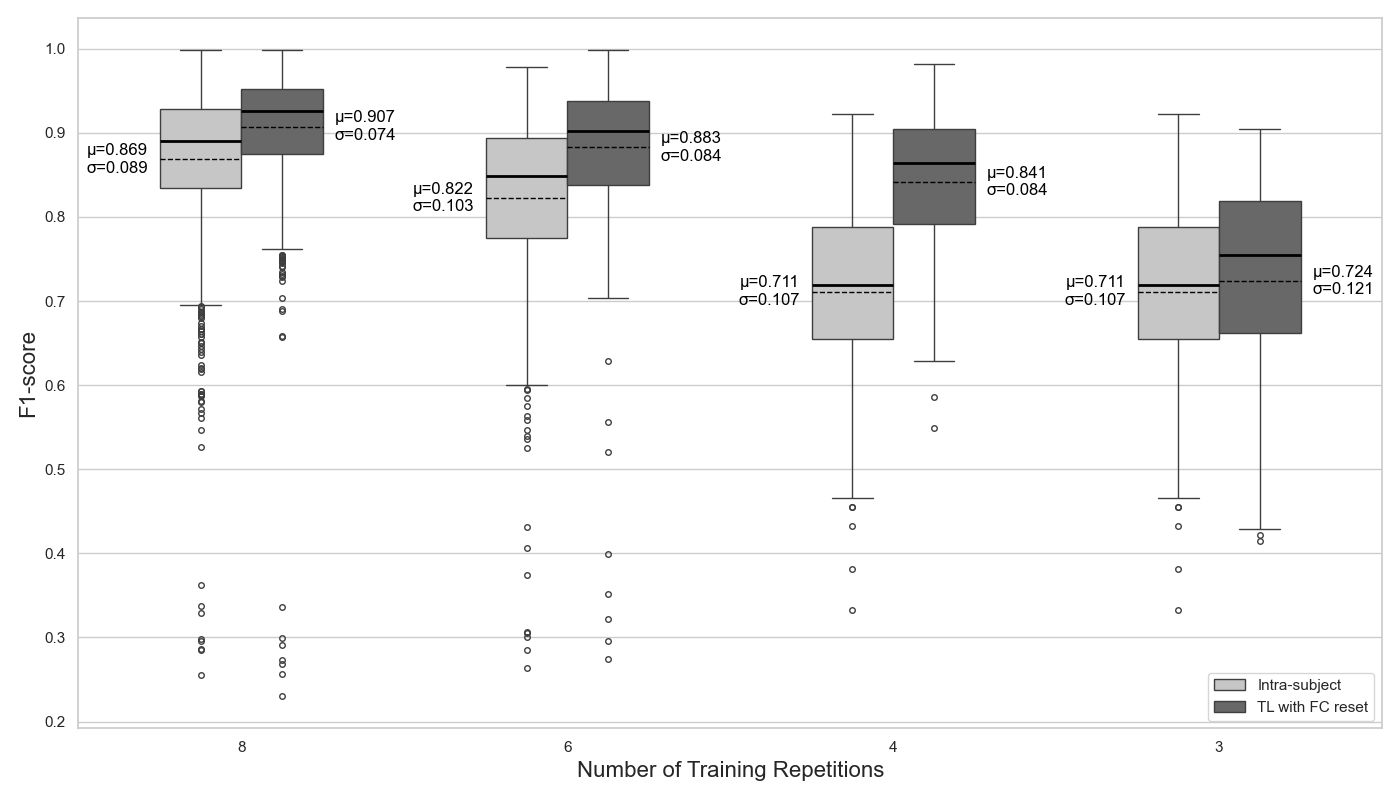
\includegraphics[width=\linewidth]{intra_subject_vs_fine_tuned_by_reps}
\captionof{figure}{Box-and-whisker plots showing the distribution of F1-scores across different numbers of training repetitions (6, 4, 2, 1) for intra-subject training and transfer learning (with fully connected layer reset). Note that repetitions numbers here represent a total number of repetitions consisting of eleven gestures a subject would need to execute. Each box shows the interquartile range and median; dashed lines denote the mean. Outliers are plotted as individual points.}
\label{fig:boxplot-reps}
\end{center}
\begin{multicols}{2}

\subsection*{Statistical Significance of Transfer Learning Improvements}

To formally test the impact of transfer learning approaches, we performed Wilcoxon signed-rank tests on the subject-wise mean and standard deviation (STD) of F1-scores. The significance level was set to $\alpha = 0.05$.

\textbf{Comparison: Intra-subject (8 repetitions) vs Transfer Learning (without FC reset, 8 repetitions).}  
The mean F1-score increased from $0.869$ to $0.896$. Wilcoxon test ($p = 7.87 \times 10^{-6}$) confirmed a statistically significant improvement. However, the decrease in STD from 0.089 to 0.071 was not statistically significant ($p = 0.0829$).

\textbf{Comparison: Intra-subject (8 repetitions) vs Transfer Learning (with FC reset, 8 repetitions).}  
The mean F1-score increased to $0.907$. Wilcoxon test ($p = 2.38 \times 10^{-7}$) confirmed this improvement to be statistically significant. Additionally, the reduction in STD from 0.089 to 0.074 was also statistically significant ($p = 0.00162$), indicating enhanced model stability.

\textbf{Comparison: Transfer Learning without FC (8 repetitions) vs with FC reset (8 repetitions).}  
The ``with FC reset'' strategy outperformed ``without reset'' in mean F1-score (0.907 vs 0.896), with Wilcoxon test yielding $p = 0.000346$, indicating statistical significance. The change in STD was not statistically significant ($p = 0.118$).

\textbf{Effect of Repetition Count on Statistical Significance.}  
To validate whether transfer learning with FC reset remains statistically superior to training from the scratch (intra-subject approach) when fewer training repetitions are used, Wilcoxon tests were also conducted for 6, 4, and 3 repetitions:

- \textit{6 repetitions:} F1-score improved from 0.822 to 0.883 ($p = 2 \times 10^{-5}$); STD statistically significantly reduced from 0.103 to 0.084 ($p = 0.0333$).
- \textit{4 repetitions:} F1-score improved from 0.711 to 0.841 ($p = 2 \times 10^{-5}$); STD statistically significantly reduced from 0.107 to 0.084 ($p = 0.00183$).
- \textit{3 repetitions:} F1-score improved from 0.463 to 0.724 ($p = 2 \times 10^{-5}$); STD statistically significantly reduced from 0.127 to 0.121 ($p = 0.0473$).

These results demonstrate that the benefit of transfer learning with FC reset remains statistically significant across differnet amount of available training data. This confirms its robustness and practicality for reducing subject burden during calibration.

The training results, as well as python scripts used to analyse those results are available in the publicly accessible repository~\cite{Kolomiiets2025}.

\subsection*{Summary of Findings}

In summary:
\begin{itemize}
    \item Both transfer learning strategies significantly outperform intra-subject training in classification accuracy.
    \item Transfer learning with FC reset is statistically more stable than intra-subject training.
    \item Transfer learning allows for comparable or better performance even when fine-tuning with very limited subject-specific data.
    \item Among the strategies, fine-tuning with FC reset provides the best overall performance in terms of accuracy and stability.
\end{itemize}

These findings validate the efficacy of transfer learning for sEMG gesture recognition and highlight the practical advantage of using pre-trained models for quick subject adaptation, especially in real-time or low-data scenarios.

\subsection*{Limitations, Comparison to Related Work, and Future Directions}

While the experimental results strongly support the effectiveness of transfer learning—particularly the fine-tuning with FC reset strategy—several limitations should be acknowledged.

First, the convolutional neural network (CNN) architecture employed in this study was intentionally kept relatively shallow to ensure comparability with baseline works and maintain computational simplicity~\cite{Cote2019_3DC,LibEMG2023}. However, this architecture may not fully exploit the temporal and spatial dependencies in sEMG signals. More advanced architectures, such as gated temporal convolutional networks~\cite{Xie2024} or hybrid CNN–LSTM models~\cite{Faust2018}, could potentially further improve classification performance and stability.

Second, although the 3DC dataset is a well-established benchmark, it was originally designed to simulate realistic variability in electrode placement. While this strengthens the case for evaluating inter-subject generalization, it also introduces significant variability in the training data. As a result, absolute accuracy values reported in this study may be lower than those observed in more controlled datasets.

Third, although our experiments employed leave-one-out cross-validation per subject and repetition, they were conducted in an offline setting. Future evaluations in real-time or online scenarios are necessary to validate the practicality of deploying these models in wearable systems or interactive applications~\cite{Shen2020}.

In comparison to related studies, our results are consistent with prior works by Côté-Allard et al.~\cite{Cote2019}, who demonstrated the benefits of transfer learning on sEMG-based gesture recognition. However, those studies typically used a single transfer learning strategy. Our work expands upon this by systematically comparing fine-tuning with and without FC reset and providing robust statistical analysis. Furthermore, while Lehmler et al.~\cite{Lehmler2021} and Ameri et al.~\cite{Ameri2020} investigated domain adaptation and transfer across electrode shifts, few works have directly quantified how much subject-specific data can be saved—a contribution this paper explicitly addresses.

Future research should focus on several directions:
\begin{itemize}
    \item Exploring deeper or hybrid models that can model temporal dynamics explicitly (e.g., attention-based or transformer architectures).
    \item Incorporating domain adaptation techniques to further mitigate distributional shifts between training and target subjects.
    \item Investigating few-shot or semi-supervised learning approaches to reduce calibration requirements even further.
    \item Evaluating latency and resource usage for deployment on low-power microcontrollers to ensure feasibility in wearable devices.
\end{itemize}

In addition, public benchmarking on larger and more diverse datasets would help generalize these findings to broader use cases. The proposed evaluation pipeline based on \texttt{LibEMG} and 3DC can serve as a reproducible and extensible framework for future comparisons.

\section*{Conclusion}

This study investigated the effectiveness of transfer learning for surface electromyography (sEMG) gesture classification using convolutional neural networks. By comparing intra-subject training, inter-subject generalization, and two transfer learning strategies (with and without resetting the FC layer), we demonstrated that transfer learning significantly enhances classification performance and model stability.

Our experiments showed that fine-tuning pre-trained models—especially when resetting the FC layer—not only improves F1-scores but also reduces standard deviation across cross-validation folds, indicating more consistent performance. Notably, this benefit remains statistically significant even when using a reduced number of repetitions for subject-specific fine-tuning, suggesting that transfer learning can substantially reduce the effort required for user calibration.

In addition, the statistical analysis using Wilcoxon signed-rank tests confirmed the superiority of the fine-tuned models under various data constraints. These findings emphasize the practicality of transfer learning in real-world applications where data availability is limited.

Nevertheless, the study has several limitations. The CNN architecture used is relatively simple and may not capture more complex spatiotemporal dependencies in the EMG signal. Also, evaluations were conducted in an offline setting using a single dataset (3DC), which, while realistic in variability, may not generalize to all EMG acquisition systems or environments.

Future work should explore deeper and hybrid models, real-time implementations, and domain adaptation techniques to further reduce calibration overhead. Expanding evaluation to diverse datasets and hardware platforms will be critical to validating these results at scale.

In summary, transfer learning—particularly fine-tuning with FC reset—emerges as a highly effective strategy for subject adaptation in sEMG-based gesture recognition, offering both performance improvements and practical utility for deployment in wearable systems.

\pdfbookmark[1]{References}{translit}
\renewcommand{\refname}{References}

\begin{thebibliography}{99}\footnotesize 

\bibitem{Zhou2023}
Zhou, Y., Wang, Y., Wang, X., \& Zhang, Y., 2023. Electromyography monitoring systems in rehabilitation: A review of current applications and future challenges. \textit{Electronics}, 12(7), p.1520. Available at: \url{https://doi.org/10.3390/electronics12071520} [Accessed 25 May 2025].

\bibitem{Xie2024}
Xie, P., Xu, M., Shen, T., Chen, J., Jiang, G., Xiao, J., \& Chen, X., 2024. A channel-fused gated temporal convolutional network for EMG-based gesture recognition. \textit{Biomedical Signal Processing and Control}, 95, 106408. Available at: \url{https://doi.org/10.1016/j.bspc.2024.106408} [Accessed 25 May 2025].

\bibitem{Merletti2020}
Merletti, R. \& Farina, D., 2020. Tutorial. Surface EMG detection, conditioning and pre-processing: Best practices. \textit{Journal of Electromyography and Kinesiology}, 54, p.102440. Available at: \url{https://doi.org/10.1016/j.jelekin.2020.102440} [Accessed 25 May 2025].

\bibitem{Plux2022}
Plux Biosignals, 2022. Where should I place my Electromyography (EMG) electrodes? Available at: \url{https://support.pluxbiosignals.com/knowledge-base/where-should-i-place-my-electromyography-emg-electrodes/} [Accessed 25 May 2025].

\bibitem{Chowdhury2013}
Chowdhury, R.H., Reaz, M.B.I., Ali, M.A.B.M., Bakar, A.A.A., Chellappan, K., \& Chang, T.G., 2013. Surface electromyography signal processing and classification techniques. \textit{Sensors}, 13(9), pp.12431–12466. Available at: \url{https://doi.org/10.3390/s130912431} [Accessed 25 May 2025].

\bibitem{Phinyomark2019}
Phinyomark, A., Campbell, E., \& Scheme, E., 2019. Surface electromyography (EMG) signal processing, classification, and practical considerations. In: G. Naik, ed., \textit{Biomedical Signal Processing}. Singapore: Springer, pp.3–29. Available at: \url{https://doi.org/10.1007/978-981-13-9097-5_1} [Accessed 25 May 2025].

\bibitem{Faust2018}
Faust, O., Hagiwara, Y., Hong, T.J., Lih, O.S. \& Acharya, U.R., 2018. Deep learning for healthcare applications based on physiological signals: A review. \textit{Computer Methods and Programs in Biomedicine}, 161, pp.1–13. Available at: \url{https://doi.org/10.1016/j.cmpb.2018.04.005} [Accessed 25 May 2025].

\bibitem{Wu2022}
Wu, D., Yang, J., \& Sawan, M., 2022. Transfer learning on electromyography (EMG) tasks: Approaches and beyond. \textit{arXiv preprint arXiv:2210.06295}. Available at: \url{https://arxiv.org/abs/2210.06295} [Accessed 25 May 2025].

\bibitem{Cote2019}
Côté-Allard, U., Fall, C.L., Campeau-Lecours, A., et al., 2019. Deep learning for electromyographic hand gesture signal classification using transfer learning. \textit{IEEE Transactions on Neural Systems and Rehabilitation Engineering}, 27(4), pp.760–771. Available at: \url{https://doi.org/10.1109/TNSRE.2019.2896269} [Accessed 25 May 2025].

\bibitem{Ameri2020}
Ameri, A., Akhaee, M.A., Scheme, E. \& Englehart, K.B., 2020. A deep transfer learning approach to reducing the effect of electrode shift in EMG pattern recognition-based control. \textit{IEEE Transactions on Neural Systems and Rehabilitation Engineering}, 28(2), pp.370–379. Available at: \url{https://doi.org/10.1109/TNSRE.2019.2962189} [Accessed 25 May 2025].

\bibitem{Shen2020}
Shen, S., Gu, K., Chen, X.-R., Lv, C.-X., \& Wang, R.-C., 2020. Gesture recognition through sEMG with wearable device based on deep learning. \textit{Mobile Networks and Applications}, 25(6), pp.2447–2458. Available at: \url{https://doi.org/10.1007/s11036-020-01590-8} [Accessed 25 May 2025].

\bibitem{Geng2016}
Geng, Y., Zhou, P. \& Li, G., 2016. Toward attenuating the impact of inter-session variability in myoelectric pattern recognition using adaptive sparse representation. \textit{Journal of NeuroEngineering and Rehabilitation}, 13(1), p.4. Available at: \url{https://doi.org/10.1186/s12984-015-0114-3} [Accessed 25 May 2025].

\bibitem{Lehmler2021}
Lehmler, S.J., Saif-ur-Rehman, M., Glasmachers, T. \& Iossifidis, I., 2021. Deep transfer-learning for patient specific model re-calibration: Application to sEMG-classification. \textit{arXiv preprint arXiv:2112.15019}. Available at: \url{https://arxiv.org/abs/2112.15019} [Accessed 25 May 2025].

\bibitem{Cote2019_3DC}
Côté-Allard, U., Campbell, E., Phinyomark, A., et al., 2019. A low-cost, wireless, 3D-printed custom armband for sEMG hand gesture recognition. \textit{Sensors}, 19(12), 2811. Available at: \url{https://doi.org/10.3390/s19122811} [Accessed 25 May 2025].

% Methods
\bibitem{LibEMG2023}
Campeau-Lecours, A., Bouchard, D., Côté-Allard, U. and Gosselin, B., 2023. LibEMG: An Open Source Library to Facilitate the Exploration of Myoelectric Control. \textit{IEEE Access}, 11, pp.88686–88702. Available at: \url{https://doi.org/10.1109/ACCESS.2023.3304544} [Accessed 25 May 2025].

\bibitem{Smith2011}
Smith, L.H., Hargrove, L.J., Lock, B.A. and Kuiken, T.A., 2011. Determining the optimal window length for pattern recognition-based myoelectric control: balancing the competing effects of classification error and controller delay. \textit{IEEE Transactions on Neural Systems and Rehabilitation Engineering}, 19(2), pp.186--192. Available at: \url{https://doi.org/10.1109/TNSRE.2010.2100828} [Accessed 26 May 2025].

\bibitem{Rehman2018}
Rehman, M.Z.U., Waris, A., Gilani, S.O., Jochumsen, M., Niazi, I.K., Jamil, M., Farina, D. and Kamavuako, E.N., 2018. Multiday EMG-Based Classification of Hand Motions With Deep Learning Techniques. \textit{Sensors}, 18(8), p.2497. Available at: \url{https://doi.org/10.3390/s18082497} [Accessed 25 May 2025].

\bibitem{Oskoei2007}
Oskoei, M.A. and Hu, H., 2007. Myoelectric control systems—A survey. \textit{Biomedical Signal Processing and Control}, 2(4), pp.275–294. Available at: \url{https://doi.org/10.1016/j.bspc.2007.07.009} [Accessed 25 May 2025].

\bibitem{Kolomiiets2025}
Kolomiiets, B. Yu., 2025. *Code used for experiments presented in this artcile* [online]. GitHub. Available at: \url{https://github.com/bohdan-kolomiiets/phd-article-1} [Accessed 27 May 2025].

\end{thebibliography}  

\TitleSecond{Improving sEMG Gesture Classification with Transfer Learning: Accuracy, Stability, and Low-Data Adaptation}
\Auth{Kolomiiets B. Yu., Karplyuk Ye. S.}
\AbsK{
Surface electromyography (sEMG) enables intuitive and non-invasive human–machine interfacing, yet its practical deployment remains limited by inter-subject variability and the substantial effort required for subject-specific model calibration. In this work, we evaluate the effectiveness of transfer learning to address these challenges in the context of deep learning-based gesture classification, using a dataset that includes eleven gestures repeated eight times by 22 subjects. We systematically compare three training paradigms: (i) intra-subject training, (ii) inter-subject generalization, and (iii) transfer learning with and without resetting the classifier’s fully connected (FC) output layer. A rigorous leave-one-out cross-validation scheme was applied across all subjects and repetitions to ensure robust evaluation.
Our results show that both transfer learning strategies outperform baseline models in terms of classification accuracy, with the best performance achieved when fine-tuning with a reset FC layer (F1-score = 0.907, $\sigma = 0.074$). Statistical analysis using Wilcoxon signed-rank tests confirms that these improvements are significant, even when only a limited number of subject-specific repetitions are used for fine-tuning. Notably, the transfer learning approach being trained on four repetitions maintains almost the same performance compared to training from scratch on eight repetitions, halving training repetitions while preserving accuracy. This represents a substantial reduction in calibration effort without sacrificing performance.
These findings support the use of pre-trained models for rapid subject adaptation in sEMG-controlled systems and validate fine-tuning with FC reset as an effective strategy for improving both performance and model stability. The methodology and results presented in this work contribute to the development of practical, adaptive, and low-effort EMG-based interfaces for assistive and rehabilitative applications.
}
{
surface electromyography (sEMG), gesture recognition, transfer learning, deep learning, convolutional neural networks (CNN), inter-subject variability, model generalization, fine-tuning strategies, subject adaptation, myoelectric control, EMG-based interface, cross-validation, biomedical signal processing, rehabilitation technologies, low-effort calibration
}

\label{radap20NN:LastPage}
\end{multicols}
\newpage
%%%%%%%%%%%%%  END of GENERATED TEXT  %%%%%%%%%%%%\n